\documentclass[journal]{IEEEtran}

% --- Core Packages ---
\usepackage{_internals/preamble} % Load all common packages from preamble.sty

% --- Bibliography Setup (BibLaTeX) ---
% Load biblatex *after* the class and preamble, but *before* \begin{document}
\usepackage[backend=biber,style=ieee,natbib=true, maxnames=6, minnames=1, date=year, doi=false, isbn=false, url=false]{biblatex} % Using biblatex-ieee
% Options explained:
% maxnames=6: Show up to 6 authors, then use 'et al.'
% minnames=1: Use 'et al.' if there's more than 1 author *and* maxnames is exceeded.
% date=year: Only show year, not month/day
% doi=false, isbn=false, url=false: Hide these fields by default (common for IEEE)
\addbibresource{../pustaka.bib} % Path to your master .bib file

% --- Document Specific Information (from settings.tex or defined here) ---
% %-----------------------------------------------------------------------------%
% Informasi Mengenai Dokumen
%-----------------------------------------------------------------------------%
%
% Judul laporan.
\var{\judul}{Implementasi dan Analisis Efektivitas Vxlang \f{Code Virtualization} dalam mempersulit \f{Reverse Engineering}}
%
% Tulis kembali judul laporan, kali ini akan diubah menjadi huruf kapital
\Var{\Judul}{Implementasi dan Analisis Efektivitas Vxlang \f{Code Virtualization} dalam mempersulit \f{Reverse Engineering}}
%
% Tulis kembali judul laporan namun dengan bahasa Ingris
\var{\judulInggris}{Implementation and Analysis of the Effectiveness of Vxlang Code Virtualization in complicating Reverse Engineering}
%
% Tipe laporan, dapat berisi Skripsi, Tugas Akhir, Thesis, atau Disertasi
\var{\type}{Skripsi}
%
% Tulis kembali tipe laporan, kali ini akan diubah menjadi huruf kapital
\Var{\Type}{Skripsi}
%
% Tulis nama penulis
\var{\penulis}{Seno Pamungkas Rahman}
%
% Tulis kembali nama penulis, kali ini akan diubah menjadi huruf kapital
\Var{\Penulis}{Seno Pamungkas Rahman}
%
% Tulis NPM penulis
\var{\npm}{2106731586}
%
% Tuliskan Fakultas dimana penulis berada
\Var{\Fakultas}{Teknik}
\var{\fakultas}{Teknik}
%
% Tuliskan Program Studi yang diambil penulis
\Var{\Program}{Teknik Komputer}
\var{\program}{Teknik Komputer}
%
% Tuliskan tahun publikasi laporan
\Var{\bulan}{Mei}
\Var{\tahun}{2025}
%
% Tuliskan gelar yang akan diperoleh dengan menyerahkan laporan ini
\var{\gelar}{Sarjana Teknik}
%
% Tuliskan tanggal pengesahan laporan, waktu dimana laporan diserahkan ke
% penguji/sekretariat
\var{\tanggalPengesahan}{24 Mei 2025}
%
% Tuliskan tanggal keputusan sidang dikeluarkan dan penulis dinyatakan
% lulus/tidak lulus
\var{\tanggalLulus}{24 Mei 2025}
%
% Tuliskan pembimbing
\var{\pembimbing}{Dr. Ruki Harwahyu, S.T. M.T. MSc.}
%
% Tuliskan penguji
\var{\pengujisatu}{Yan Maraden, S.T., M.T., M.Sc.}
\var{\pengujidua}{Muhammad Firdaus Syawaludin Lubis, S.T., MT., Ph.D.}
%
% Alias untuk memudahkan alur penulisan paa saat menulis laporan
\var{\saya}{Penulis}

%-----------------------------------------------------------------------------%
% Judul Setiap Bab
%-----------------------------------------------------------------------------%
%
% Berikut ada judul-judul setiap bab.
% Silahkan diubah sesuai dengan kebutuhan.
%
\Var{\kataPengantar}{Kata Pengantar}
\Var{\babSatu}{Pendahuluan}
\Var{\babDua}{Tinjauan Pustaka}
\Var{\babTiga}{Metode Penelitian}
\Var{\babEmpat}{Implementasi}
\Var{\babLima}{Hasil Penelitian}
\Var{\babEnam}{Kesimpulan dan Saran}
 % Keep if settings.tex contains commands needed ONLY here (like \judul)
                      % If commands like \Penulis are only for skripsi, remove this input.

% Define commands specifically for THIS journal paper:
\newcommand{\journalTitle}{Implementation and Analysis of Code Virtualization Effectiveness using VxLang for Mitigating Reverse Engineering}
\newcommand{\authorOne}{Seno Pamungkas Rahman}
\newcommand{\authorOneAffiliation}{Department of Electrical Engineering, Faculty of Engineering, Universitas Indonesia, Depok, 16424, Indonesia} % Added postal code
\newcommand{\authorOneEmail}{seno.pamungkas@ui.ac.id}
% \newcommand{\authorTwo}{Dr. Ruki Harwahyu, S.T., M.T., M.Sc.} % Example for Advisor
% \newcommand{\authorTwoAffiliation}{Dept. of Electrical Engineering, Fac. of Engineering, Universitas Indonesia} % Keep affiliations consistent
% \newcommand{\authorTwoEmail}{ruki.harwahyu@ui.ac.id} % Example email
\newcommand{\correspondingAuthor}{Seno Pamungkas Rahman}




% --- Start of Document ---
\begin{document}

% --- Paper Title ---
\title{\journalTitle}

% --- Author Information ---
\author{\IEEEauthorblockN{\authorOne\IEEEauthorrefmark{1}} % Use refmark if needed for affiliations/notes
        % , \IEEEauthorblockN{Author Two Name\IEEEauthorrefmark{2}} % Add other authors
\IEEEauthorblockA{\textit{\authorOneAffiliation} \\ Email: \authorOneEmail}
% \IEEEauthorblockA{\IEEEauthorrefmark{2}\textit{Affiliation Author Two}} % Corresponding affiliation
% --- Add more authors/affiliations as needed ---

\thanks{Manuscript received Month DD, YYYY; revised Month DD, YYYY. This work was supported in part by [Funding Agency, Grant Number, if any]. (Corresponding author: \correspondingAuthor.)} % Update or remove as appropriate
% \thanks{\authorOne is with the Department of Electrical Engineering, Faculty of Engineering, Universitas Indonesia, Depok, 16424 Indonesia (e-mail: \authorOneEmail).} % Standard IEEE affiliation format
% \thanks{Author Two is with ...} % Add other author affiliations if needed
}

% --- Paper Headers ---
% Optional: Customize headers for published version/preprint
% \markboth{IEEE Transactions on Dependable and Secure Computing,~Vol.~XX, No.~XX, Month~YYYY}%
% {Rahman: Analysis of VxLang Code Virtualization Effectiveness}

% --- Make Title Area ---
\maketitle

% --- Abstract and Keywords ---
\begin{abstract}
Reverse engineering poses a significant threat to software security, enabling attackers to analyze, understand, and illicitly modify program code. Code obfuscation techniques, particularly code virtualization, offer a promising defense mechanism. This paper presents an implementation and analysis of the effectiveness of code virtualization using the VxLang framework in enhancing software security against reverse engineering. We applied VxLang's virtualization to critical sections of case study applications, including authentication logic. Static analysis using Ghidra and dynamic analysis using x64dbg were performed on both the original and virtualized binaries. The results demonstrate that VxLang significantly increases the complexity of reverse engineering. Static analysis tools struggled to disassemble and interpret the virtualized code, failing to identify instructions, functions, or meaningful data structures. Dynamic analysis was similarly hampered, with obfuscated control flow and the virtual machine's execution model obscuring runtime behavior and hindering debugging attempts. However, this enhanced security comes at the cost of substantial performance overhead, observed in QuickSort algorithm execution and AES encryption benchmarks, along with a significant increase in executable file size. The findings confirm that VxLang provides robust protection against reverse engineering but necessitates careful consideration of the performance trade-offs for practical deployment.
\end{abstract}

\begin{IEEEkeywords}
Code Obfuscation, Code Virtualization, Software Protection, Reverse Engineering, VxLang, Security Analysis, Performance Overhead.
\end{IEEEkeywords}


% --- Main Content ---
\IEEEpeerreviewmaketitle % Command for peer review markers

\section{Introduction}
\IEEEPARstart{T}{he} rapid advancement of software technology has led to increasingly sophisticated applications, yet this progress is paralleled by evolving security threats. Reverse engineering, the process of analyzing software to understand its internal workings without access to source code or original designs \cite{Has18}, represents a critical vulnerability. Attackers leverage reverse engineering to uncover proprietary algorithms, identify security flaws, bypass licensing mechanisms, pirate software, and inject malicious code \cite{Wak24}. Traditional security measures like data encryption or password protection often prove insufficient against determined reverse engineers who can analyze the program's logic once it is running \cite{Sec19}.

To counter this threat, code obfuscation techniques aim to transform program code into a functionally equivalent but significantly harder-to-understand form \cite{Jin24}. Among various obfuscation strategies, code virtualization stands out as a particularly potent approach \cite{Ore06, Zho24}. This technique translates native machine code into custom bytecode instructions executed by a dedicated virtual machine (VM) embedded within the application \cite{Don20}. The unique Instruction Set Architecture (ISA) of this VM renders conventional reverse engineering tools like disassemblers and debuggers largely ineffective, as they cannot directly interpret the virtualized code \cite{Salwan2018SymbolicDeobfuscation}. Attackers must first decipher the VM's architecture and bytecode, substantially increasing the effort and complexity required for analysis \cite{Hac24}.

VxLang is a code protection framework that incorporates code virtualization capabilities, targeting Windows PE executables \cite{VxLang}. It provides mechanisms to transform native code into its internal bytecode format, executed by its embedded VM. Understanding the practical effectiveness and associated costs of such tools is crucial for developers seeking robust software protection solutions.

This paper investigates the effectiveness of code virtualization using VxLang in mitigating reverse engineering efforts. We aim to answer the following key questions:
\begin{enumerate}
    \item How effectively does VxLang's code virtualization obscure program logic against static and dynamic reverse engineering techniques?
    \item What is the quantifiable impact of VxLang's virtualization on application performance (execution time) and file size?
\end{enumerate}

To address these questions, we implement VxLang's virtualization on selected functions within case study applications (simulating authentication) and performance benchmarks (QuickSort, AES encryption). We then perform comparative static analysis (using Ghidra \cite{Nat19}) and dynamic analysis (using x64dbg \cite{Dun14}) on the original and virtualized binaries. Performance overhead is measured by comparing execution times and executable sizes, and the impact on automated malware detection tools is assessed using VirusTotal analysis on a relevant case study.

The primary contributions of this work are:
\begin{itemize}
    \item A practical implementation and evaluation of VxLang's code virtualization on representative code segments.
    \item Qualitative and quantitative analysis of the increased difficulty imposed on static and dynamic reverse engineering by VxLang.
    \item Measurement and analysis of the performance and file size overhead associated with VxLang's virtualization.
    \item An empirical assessment of the security-performance trade-off offered by the VxLang framework.
\end{itemize}

The remainder of this paper is organized as follows: Section \ref{sec:related_work} discusses related work in code obfuscation and virtualization. Section \ref{sec:methodology} details the methodology employed in our experiments. Section \ref{sec:implementation} briefly outlines the implementation setup. Section \ref{sec:results_discussion} presents and discusses the experimental results for both security and performance analysis. Finally, Section \ref{sec:conclusion} concludes the paper and suggests directions for future research.

\section{Related Work} \label{sec:related_work}
Protecting software from unauthorized analysis and tampering is a long-standing challenge. Reverse engineering techniques are constantly evolving, necessitating more sophisticated protection mechanisms. This section reviews relevant work in code obfuscation, focusing on code virtualization.

\subsection{Code Obfuscation Techniques}
Obfuscation aims to increase the complexity of understanding code without altering its functionality \cite{Jin24}. Techniques operate at different levels:

\subsubsection{Source Code Obfuscation} Modifies the human-readable source code.
\begin{itemize}
    \item \textbf{Layout Obfuscation:} Alters code appearance (e.g., scrambling identifiers \cite{Cha04}, removing comments/whitespace \cite{Bal11}). Provides minimal security against automated tools.
    \item \textbf{Data Obfuscation:} Hides data representation (e.g., encoding strings \cite{Ert05, Fuk08, Kov13}, splitting/merging arrays, using equivalent but complex data types). Can make data analysis harder. Techniques like instruction substitution \cite{LeD12, Dar10} and mixed boolean-arithmetic \cite{Liu21, Sch22, Zho07} fall under this category, obscuring data manipulation logic.
    \item \textbf{Control Flow Obfuscation:} Modifies the program's execution path logic. Examples include inserting bogus control flow \cite{LiY211}, using opaque predicates (conditional statements whose outcome is known at obfuscation time but hard to determine statically \cite{XuD16}), and control flow flattening, which transforms structured code into a large switch statement, obscuring the original logic \cite{Lás09}.
\end{itemize}

\subsubsection{Bytecode Obfuscation} Targets intermediate code (e.g., Java bytecode, .NET CIL, LLVM IR). Techniques include renaming identifiers, control flow obfuscation, string encryption, and inserting dummy code \cite{Pie18, Yak20}. Effective against decompilation back to high-level source code.

\subsubsection{Binary Code Obfuscation} Operates on the final machine-executable code.
\begin{itemize}
    \item \textbf{Code Packing/Encryption:} Compresses or encrypts the original code, requiring a runtime stub to unpack/decrypt it before execution \cite{Rou13}. Primarily hinders static analysis but reveals the original code in memory during execution.
    \item \textbf{Control Flow Manipulation:} Uses indirect jumps/calls, modifies call/ret instructions, or chunks code into small blocks with jumps to disrupt linear disassembly and analysis \cite{Rou13}.
    \item \textbf{Constant Obfuscation:} Hides constant values through arithmetic/logical operations \cite{Rou13}.
    \item \textbf{Code Virtualization:} As discussed below, this is considered one of the strongest binary obfuscation techniques.
\end{itemize}

\subsubsection{Disassembly Techniques and Challenges}
Understanding the efficacy of binary obfuscation, particularly code virtualization, necessitates a brief overview of disassembly techniques. Disassemblers translate machine code into human-readable assembly language, forming a cornerstone of reverse engineering \cite{Sikorski2012}. Two primary approaches exist: static and dynamic disassembly.

Static disassemblers, such as Ghidra \cite{Nat19} and IDA Pro \cite{Hex91}, analyze executable files without running them. They employ techniques like linear sweep or recursive traversal to identify instruction sequences \cite{Eilam2011, Ko2007}. While comprehensive, static analysis struggles with code that is encrypted, packed, self-modifying, or significantly transformed, as the disassembler may misinterpret data as code or fail to follow the true control flow \cite{Sikorski2012, Blazytko2017}. Crucially, when faced with custom bytecode from a virtual machine (VM), static disassemblers designed for standard ISAs (e.g., x86-64) cannot correctly interpret these non-native instructions, leading to analysis failure.

Dynamic disassembly, typically a feature of debuggers like x64dbg \cite{Dun14}, occurs during program execution. The debugger disassembles instructions on-the-fly as they are about to be executed by the CPU. This approach can overcome some static analysis limitations, such as revealing unpacked or decrypted code in memory \cite{Sikorski2012}. Debuggers can also access runtime symbol information loaded by the operating system for system libraries, providing context for API calls. However, while a debugger can step through the native instructions of an embedded VM's interpreter, it will not directly reveal the original, pre-virtualized logic of the application. Instead, it shows the VM's internal operations executing the custom bytecode, which still obscures the application's core semantics from the analyst. These inherent limitations of standard disassembly tools underscore the challenge posed by advanced obfuscation techniques like code virtualization.

\subsection{Code Virtualization (VM-Based Obfuscation)}
Code virtualization translates native code into a custom bytecode format, executed by an embedded virtual machine (VM) \cite{Ore06, Zho24}. This creates a significant barrier for reverse engineers, as standard tools cannot interpret the custom ISA \cite{Sal18}. The attacker must first understand the VM's architecture, handler implementations, and bytecode mapping, which is a complex and time-consuming task \cite{Don20, Hac24}.

Key aspects of VM-based obfuscation include:
\begin{itemize}
    \item \textbf{Custom ISA:} Each protected application can potentially have a unique or mutated set of virtual instructions, hindering signature-based detection or analysis reuse. Oreans highlights the possibility of generating diverse VMs for different protected copies \cite{Ore06}.
    \item \textbf{VM Architecture:} Typical VM components include fetch, decode, dispatch, and handler units, mimicking CPU operations but implemented in software \cite{Sal18, Hac24}. The complexity and implementation details of these handlers directly impact both security and performance.
    \item \textbf{Security vs. Performance Trade-off:} The interpretation layer introduced by the VM inherently adds performance overhead compared to native execution. The level of obfuscation within the VM handlers and the complexity of the virtual instructions influence this trade-off.
\end{itemize}

Several commercial tools like VMProtect \cite{VMP24} and Themida \cite{Ore24} (which also includes virtualization features beyond basic packing) employ code virtualization. Academic research has also explored techniques like symbolic deobfuscation to analyze virtualized code \cite{Sal18} and methods to enhance virtualization robustness, such as virtual code folding \cite{Don20}.

\subsection{VxLang in Context}
VxLang positions itself as a comprehensive framework offering binary protection, code obfuscation (including flattening), and code virtualization \cite{VxLang}. Its approach involves transforming native x86-64 code into an internal bytecode executed by its VM. This study aims to provide an empirical evaluation of the effectiveness of VxLang's virtualization component against standard reverse engineering practices and quantify its associated performance costs, contributing practical insights into its utility as a software protection mechanism. Unlike analyzing established commercial protectors, this work focuses on the specific implementation and impact of the VxLang framework.

\section{Methodology} \label{sec:methodology}
This research employs an experimental approach to evaluate the effectiveness of VxLang's code virtualization. We compare the reverse engineering difficulty and performance characteristics of software binaries before and after applying VxLang's virtualization.

\subsection{Experimental Design}
A comparative study design was used, involving a control group (original, non-virtualized binaries) and an experimental group (binaries with critical sections virtualized by VxLang).

\begin{itemize}
    \item \textbf{Independent Variable:} Application of VxLang code virtualization (Applied vs. Not Applied).
    \item \textbf{Dependent Variables:}
        \begin{itemize}
            \item \textit{Reverse Engineering Difficulty:} Qualitatively assessed based on the effort required for static analysis (code understanding, logic identification, patching attempts using Ghidra) and dynamic analysis (runtime tracing, memory inspection, manipulation attempts using x64dbg). Success/failure of bypassing authentication logic was recorded.
            \item \textit{Performance Overhead:} Quantitatively measured via execution time for specific computational tasks (QuickSort, AES encryption/decryption).
            \item \textit{File Size Overhead:} Quantitatively measured by comparing the size (in bytes) of the final executable files.
        \end{itemize}
\end{itemize}

\subsection{Study Objects}
Two categories of applications were developed and analyzed:

\subsubsection{Authentication Case Study Applications} Simple applications simulating user login were created to serve as targets for reverse engineering analysis focused on bypassing the authentication mechanism. Variants included:
    \begin{itemize}
        \item \textbf{Interface Types:} Console (CLI), Qt Widgets (GUI), Dear ImGui (Immediate Mode GUI).
        \item \textbf{Authentication Mechanisms:} Hardcoded credentials (comparing input against string literals) and Cloud-based validation (sending credentials via HTTP POST to a local backend server).
    \end{itemize}
    For each variant, the core authentication logic (comparison function or the call to the cloud request function and subsequent result check) was targeted for virtualization in the experimental group.

\subsubsection{Performance Benchmark Applications} Applications designed to measure the performance impact of virtualization on specific computational tasks:
    \begin{itemize}
        \item \textbf{QuickSort Benchmark:} Implemented a standard recursive QuickSort algorithm. The core recursive function was virtualized. Tested with varying array sizes (100 to 1,000,000 elements).
        \item \textbf{AES Encryption Benchmark:} Implemented AES-256-CBC encryption/decryption using OpenSSL's EVP API. The loop performing batch encryption/decryption operations on 1GB of data was virtualized.
        \item \textbf{File Size Benchmark:} A minimal application with embedded dummy data to assess the baseline size increase due to the inclusion of the VxLang runtime.
    \end{itemize}

\subsubsection{Case Study: Lilith RAT}
To further evaluate VxLang's effectiveness on more complex software potentially exhibiting malicious characteristics and to assess its impact on automated detection tools, a Remote Administration Tool (RAT) named Lilith \cite{LilithRAT} was included as an additional study object. The client component of this open-source C++ RAT was compiled and analyzed both in its original form and after applying VxLang virtualization to its core functions. Analysis focused on static/dynamic reverse engineering difficulty, functional integrity post-virtualization, and detection rates by antivirus engines via VirusTotal. The Lilith server component remained unmodified and was used for functional testing of the client.

\subsection{Instrumentation and Materials}
\begin{itemize}
    \item \textbf{Hardware:} Standard Windows 11 (64-bit) PC.
    \item \textbf{Development Tools:} Clang/clang-cl (C++17), CMake, Ninja, Neovim.
    \item \textbf{Libraries/Frameworks:} VxLang SDK, Qt 6, Dear ImGui (+GLFW/OpenGL3 backend), OpenSSL 3.x, libcurl, nlohmann/json.
    \item \textbf{Analysis Tools:} Ghidra (v11.x) for static analysis, x64dbg (latest snapshot) for dynamic analysis.
    \item \textbf{Performance Measurement:} C++ \texttt{std::chrono::high\_resolution\_clock} for timing, \texttt{std::filesystem::file\_size} for file size.
\end{itemize}


\subsection{Data Collection Procedure}

\subsubsection{Security Analysis}
For each authentication application (original and virtualized):
    \begin{enumerate}
        \item \textbf{Static Analysis (Ghidra):} Load executable, search for relevant strings (e.g., "Failed", "Authorized", potential credentials), analyze disassembly/decompilation around string references or entry points, identify conditional jumps controlling authentication success/failure, attempt static patching to bypass logic. Record qualitative observations on difficulty.
        \item \textbf{Dynamic Analysis (x64dbg):} Run executable under debugger, search for strings/patterns at runtime, set breakpoints at suspected logic locations (identified via static analysis or runtime observation), step through execution, observe register/memory values, attempt runtime manipulation (patching conditional jumps) to bypass authentication. Record qualitative observations and success/failure of bypass attempts.
    \end{enumerate}

\subsubsection{Performance Analysis}
For each benchmark application (original and virtualized):
    \begin{enumerate}
        \item \textbf{Execution Time:} Run QuickSort benchmark 100 times per data size, record individual times. Run AES benchmark on 1GB data, record total encryption/decryption time. Use \texttt{std::chrono}. Calculate average, standard deviation (for QuickSort), and throughput (for AES).
        \item \textbf{File Size:} Measure the size of the final executable file in bytes using \texttt{std::filesystem::file\_size}.
    \end{enumerate}

\subsubsection{Lilith RAT Analysis}
\label{subsubsec:methodology_lilith_rat_journal} 
For the Lilith RAT client (original and virtualized):
\begin{enumerate}
    \item \textbf{Functional Integrity Testing:} The virtualized client was tested for core RAT functionalities (connection to server, remote command execution, file system access) against an unmodified server on a local network (client IP: \texttt{192.168.1.15}, server IP: \texttt{192.168.1.235} on port \texttt{1337}) to ensure virtualization did not break essential operations. A test file (\texttt{password.txt} containing \texttt{"THIS IS A SECRET"}) on the client machine was used to verify remote file access.
    \item \textbf{Security Analysis:} Similar static (Ghidra) and dynamic (x64dbg) analysis techniques as applied to authentication applications were used to assess reverse engineering difficulty of the RAT's core logic.
    \item \textbf{VirusTotal Analysis:} Both original and virtualized client executables were submitted to VirusTotal to compare detection rates and threat characterizations by various antivirus engines.
\end{enumerate}

\subsection{Data Analysis Techniques}
\begin{itemize}
    \item \textbf{Qualitative Security Data:} Descriptive analysis based on observation notes comparing the reverse engineering effort and success rates between control and experimental groups for both static and dynamic analysis phases.
    \item \textbf{Quantitative Performance Data:} Calculation of descriptive statistics (mean, standard deviation), percentage overhead for execution time, throughput calculation (MB/s), and percentage increase in file size. Comparative tables and graphs will be used for presentation.
    \item \textbf{Trade-off Analysis:} Synthesis of security findings and performance results to evaluate the balance between protection enhancement and performance/size costs introduced by VxLang.
\end{itemize}


\section{Implementation Details} \label{sec:implementation}
This section briefly outlines the key aspects of the experimental setup and the integration of VxLang.

\subsection{Development Environment}
All development and testing were conducted on a Windows 11 (64-bit) system. The Clang compiler (v19.1.3, via \texttt{clang-cl} for MSVC ABI compatibility) targeting x86-64 was used with the C++17 standard. CMake (v3.31) and Ninja (v1.12.1) managed the build process. Essential libraries included the VxLang SDK, Qt 6, Dear ImGui, OpenSSL 3.x, and libcurl, linked appropriately via CMake.

\subsection{VxLang Integration}
VxLang was applied to the target applications using its Software Development Kit (SDK) and external processing tool.

\subsubsection{Code Marking} Critical code sections intended for virtualization were demarcated in the C++ source code using the SDK's macros, primarily \texttt{VL\_VIRTUALIZATION\_BEGIN} and \texttt{VL\_VIRTUALIZATION\_END}. For instance, in the authentication logic:

\begin{verbatim}
    // ... Input username/password ...
    #ifdef USE_VL_MACRO
    VL_VIRTUALIZATION_BEGIN; // Mark start
    #endif

    if (check_credentials(username, password)) {
        // Authorized path
    } else {
        // Unauthorized path
    }

    #ifdef USE_VL_MACRO
    VL_VIRTUALIZATION_END; // Mark end
    #endif
    // ...
\end{verbatim}
Similar macros were placed around the recursive \texttt{quickSort} function body and the main encryption/decryption loop in the AES benchmark.

\subsubsection{Build Process} The CMake configuration was set up to generate two distinct build types:
\begin{enumerate}
    \item \textbf{Original Build:} Compiled without the \texttt{USE\_VL\_MACRO} preprocessor definition and without linking the VxLang library. Produces the baseline executable (e.g., \texttt{app\_qt.exe}).
    \item \textbf{Intermediate Build (VM Marked):} Compiled with \texttt{USE\_VL\_MACRO} defined and linked against \texttt{vxlib64.lib}. Produces an intermediate executable containing the VxLang markers (e.g., \texttt{app\_qt\_vm.exe}).
\end{enumerate}

\subsubsection{Virtualization Processing} The intermediate executables (e.g., \texttt{app\_qt\_vm.exe}) were then processed offline by the external VxLang command-line tool. This tool reads a JSON configuration file specifying input/output paths and virtualization options (e.g., virtualizing the entry point). The tool modifies the intermediate executable in-place or creates a new output file, replacing the native code within the marked sections with its virtualized bytecode and embedding the necessary VM runtime. The resulting file is the final virtualized executable used for testing. A simplified JSON configuration might look like:

\begin{verbatim}
{
  "Input": "path/to/intermediate_app_vm.exe",
  "Output": "path/to/final_virtualized_app.exe",
  "Virtualizer": {
    "EntryPoint": false 
  },
  "Obfuscator": { 
    "EntryPoint": false 
  },
  "Packer": { 
    "Enable": false 
  } 
  // Other options omitted for brevity
}
\end{verbatim}
For this study, default virtualization settings were primarily used after marking the code sections.

\section{Results and Discussion} \label{sec:results_discussion}
This section presents the results of the security analysis and performance measurements, followed by a discussion of the findings.

\subsection{Security Analysis Results}
The effectiveness of VxLang virtualization was evaluated through static and dynamic analysis attempts to understand and bypass the authentication logic in the case study applications.

\subsubsection{Static Analysis (Ghidra)}
\begin{itemize}
	\item \textbf{Non-Virtualized Binaries:} Analysis was straightforward. Relevant strings (e.g., "Authentication Failed", hardcoded "seno", "rahman") were easily located in the `.rdata` or `.text` sections. Cross-references led directly to the authentication functions. Disassembly clearly showed standard comparison instructions (\texttt{memcmp}, \texttt{strcmp}, or C++ string comparison operators) followed by conditional jumps (\texttt{JNZ}, \texttt{JE}) controlling the flow based on the comparison result (See example Listing \ref{lst:asm_static_nonvirt_snippet} and context in Appendix Listing \ref{lst:asm_static_nonvirt_full}). For cloud variants, the call to the request function and the subsequent check on its return value were identifiable (Listing \ref{lst:asm_static_cloud_snippet}, Appendix \ref{lst:asm_static_cloud_full}). Static patching of the conditional jump instruction to force the "authorized" path was trivial in all non-virtualized cases.
	\item \textbf{Virtualized Binaries:} Static analysis proved significantly more challenging.
	      \begin{itemize}
		      \item \textit{Instruction Recognition Failure:} Ghidra consistently failed to recognize standard x86-64 instructions within the virtualized sections, reporting large blocks of unknown opcodes or '???' entries. Analysis summaries showed a drastic reduction (often to zero) in the count of recognized instructions and functions compared to the originals (e.g., Fig. \ref{fig:ghidra_summary_qt_journal} vs. Fig. \ref{fig:ghidra_summary_qt_vm_journal}).
		      \item \textit{Data Obfuscation:} Critical strings like "Authentication Failed" or hardcoded credentials were no longer present as plain text in the binary, preventing simple string searches from locating the relevant code sections. Symbol information was also heavily stripped.
		      \item \textit{Control Flow Obscurity:} The clear structure of conditional checks and jumps seen in the original code was replaced by opaque sequences of seemingly unrelated or unknown instructions, making it impossible to identify the core authentication logic or the specific conditional jump to patch statically. The control flow graph became fragmented and uninformative within the virtualized regions.
	      \end{itemize}
	      Static bypass attempts were unsuccessful due to the inability to locate and understand the relevant control flow logic.
\end{itemize}

% --- Ghidra Summary Figures (Journal) ---
\begin{figure}[!t]
	\centering
	\includegraphics[width=0.9\linewidth]{../assets/pics/app_qt_summary_result.jpeg}
	\caption{Ghidra Analysis Summary for \texttt{app\_qt.exe} (Non-Virtualized).}
	\label{fig:ghidra_summary_qt_journal}
\end{figure}

\begin{figure}[!t]
	\centering
	\includegraphics[width=0.9\linewidth]{../assets/pics/app_qt_vm_summary_result.jpeg}
	\caption{Ghidra Analysis Summary for \texttt{app\_qt\_vm.exe} (Virtualized, showing data for app\_qt\_vxm.exe structure).}
	\label{fig:ghidra_summary_qt_vm_journal}
\end{figure}


\subsubsection{Dynamic Analysis (x64dbg)}
\begin{itemize}
	\item \textbf{Non-Virtualized Binaries:} Dynamic analysis corroborated static findings. Setting breakpoints based on string references or near conditional jumps identified statically was effective. Stepping through the code clearly showed the comparison logic and the conditional jump execution. Runtime patching of the jump instruction in x64dbg successfully bypassed authentication (See example Listing \ref{lst:asm_dynamic_nonvirt_snippet} and context in Appendix Listing \ref{lst:asm_dynamic_nonvirt_full}).
	\item \textbf{Virtualized Binaries:} Dynamic analysis faced significant hurdles.
	      \begin{itemize}
		      \item \textit{String Searching Failure:} Searching for relevant strings in memory during runtime often failed, similar to static analysis.
		      \item \textit{Execution Flow Tracking Difficulty:} Stepping through the virtualized code sections was extremely difficult. The instruction pointer (RIP) often appeared to loop within small blocks or jump to seemingly random locations, consistent with execution being handled by the VM interpreter rather than direct native execution (See Listings \ref{lst:asm_dynamic_io_nonvirt_snippet} vs. \ref{lst:asm_dynamic_io_virt_snippet}, Appendix \ref{lst:asm_dynamic_io_comparison_full}). Standard debugging techniques like setting breakpoints based on expected native instructions became unreliable.
		      \item \textit{State Obfuscation:} Understanding the program's state (relevant variable values, comparison results) was hindered because the actual logic was executed within the VM's context, which was not directly visible or interpretable through the debugger's view of native registers and memory.
	      \end{itemize}
	      Dynamic bypass attempts by patching suspected native jump instructions (if any could be identified near the VM entry/exit) were unsuccessful, as the core logic resided within the VM's execution loop.
\end{itemize}

These results strongly indicate that VxLang's code virtualization effectively hinders both static and dynamic reverse engineering attempts using standard tools and techniques.

\subsubsection{Analysis of Lilith RAT}
Static and dynamic analysis were also performed on the Lilith RAT client (original vs. virtualized). Findings mirrored those from the authentication case studies:
\begin{itemize}
	\item \textbf{Non-Virtualized:} Analysis was feasible. Strings related to commands and functionality were identifiable. Control flow for network communication and command handling could be traced using Ghidra and x64dbg, allowing potential understanding of its mechanisms (e.g., keylogging, remote execution).
	\item \textbf{Virtualized:} Analysis difficulty increased significantly. Ghidra failed to properly disassemble virtualized sections, showing numerous '???' entries and obscuring the logic. Dynamic tracing in x64dbg was severely hampered by the VM execution, making it hard to follow command processing or data flow.
	\item \textbf{Functional Integrity:} Importantly, functional testing confirmed that the virtualized Lilith client remained fully operational, successfully connecting to the server and executing core RAT commands, despite the code transformation.
\end{itemize}
This indicates VxLang's virtualization hinders analysis even for complex, potentially malicious software, without necessarily breaking its intended functionality.

\subsection{Performance and Size Overhead Results}

\subsubsection{Execution Time Overhead}
The performance impact was measured using QuickSort and AES benchmarks.

\begin{itemize}
	\item \textbf{QuickSort:} As shown in Table \ref{tab:quick_sort_performance_journal} and Fig. \ref{fig:quick_sort_performance_journal}, virtualization introduced substantial execution time overhead. The overhead increased with data size, ranging from approximately 27,300\% for 100 elements (0.01 ms to 2.74 ms) to about 15,150\% for 1,000,000 elements (218.32 ms to 33,292.91 ms). This indicates a significant constant overhead plus a scaling factor imposed by the VM's interpretation loop for the recursive sorting function.
	      \begin{table}[!t]
		      \centering
		      \caption{Quick Sort Execution Time Results (ms)}
		      \label{tab:quick_sort_performance_journal}
		      \resizebox{\columnwidth}{!}{%
			      \begin{tabular}{@{}lrrrr@{}}
				      \toprule
				      \multirow{2}{*}{\textbf{Array Size}} & \multicolumn{2}{c}{\textbf{Non-Virtualized}} & \multicolumn{2}{c}{\textbf{Virtualized}}                                        \\
				      \cmidrule(lr){2-3} \cmidrule(lr){4-5}
				                                           & \textbf{Avg Time}                            & \textbf{Std Dev}                         & \textbf{Avg Time} & \textbf{Std Dev} \\
				      \midrule
				      100                                  & 0.01                                         & 0.00                                     & 2.74              & 0.38             \\
				      1,000                                & 0.08                                         & 0.00                                     & 27.35             & 1.25             \\
				      5,000                                & 0.54                                         & 0.05                                     & 144.44            & 8.25             \\
				      10,000                               & 1.24                                         & 0.08                                     & 295.77            & 13.68            \\
				      50,000                               & 6.98                                         & 0.51                                     & 1,556.15          & 122.81           \\
				      100,000                              & 15.12                                        & 1.26                                     & 3,080.30          & 303.02           \\
				      500,000                              & 104.44                                       & 7.30                                     & 14,298.92         & 374.98           \\
				      1,000,000                            & 218.32                                       & 8.10                                     & 33,292.91         & 4,342.93         \\
				      \bottomrule
			      \end{tabular}
		      } % End resizebox
	      \end{table}

	      \begin{figure}[!t]
		      \centering
		      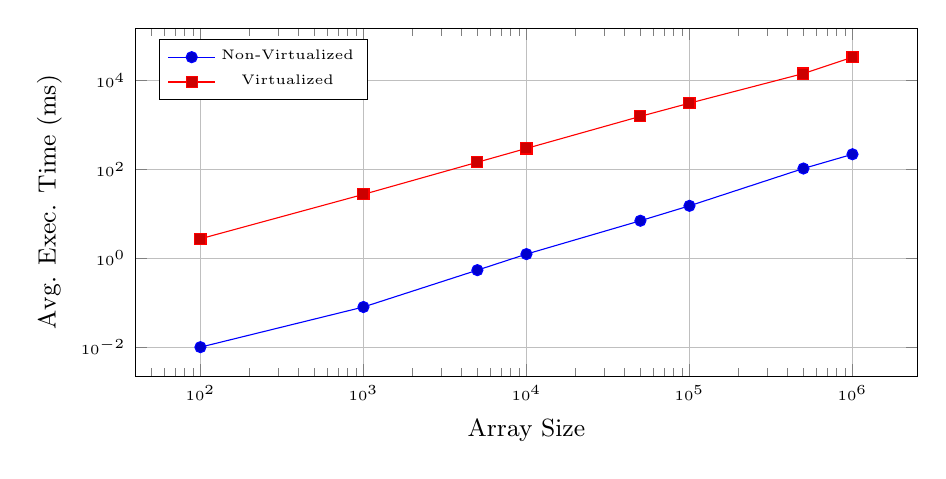
\begin{tikzpicture}
			      \begin{axis}[
					      width=0.95\columnwidth,
					      height=6cm,
					      xlabel={Array Size},
					      ylabel={Avg. Exec. Time (ms)},
					      xmode=log,
					      log basis x={10},
					      ymode=log,
					      log basis y={10},
					      legend pos=north west,
					      grid=major,
					      tick label style={font=\tiny},
					      label style={font=\small},
					      legend style={font=\tiny}
				      ]
				      \addplot coordinates {
						      (100, 0.01)
						      (1000, 0.08)
						      (5000, 0.54)
						      (10000, 1.24)
						      (50000, 6.98)
						      (100000, 15.12)
						      (500000, 104.44)
						      (1000000, 218.32)
					      };
				      \addlegendentry{Non-Virtualized};

				      \addplot coordinates {
						      (100, 2.74)
						      (1000, 27.35)
						      (5000, 144.44)
						      (10000, 295.77)
						      (50000, 1556.15)
						      (100000, 3080.30)
						      (500000, 14298.92)
						      (1000000, 33292.91)
					      };
				      \addlegendentry{Virtualized};
			      \end{axis}
		      \end{tikzpicture}
		      \caption{Quick Sort Execution Time Comparison (Log-Log Scale).}
		      \label{fig:quick_sort_performance_journal}
	      \end{figure}


	\item \textbf{AES Encryption:} Table \ref{tab:aes_performance_journal} shows that the total time for encrypting 976MB of data increased by approximately 396.7\% (1878.52 ms to 9330.73 ms), and decryption time increased by about 562.9\% (1304.75 ms to 8649.74 ms). Consequently, the combined throughput dropped dramatically from 634.16 MB/s to 108.78 MB/s (an 82.8\% reduction). This confirms a significant overhead for cryptographic operations.
	      \begin{table}[!t]
		      \centering
		      \caption{AES-256-CBC Performance Results (976MB Data)}
		      \label{tab:aes_performance_journal}
		      \resizebox{\columnwidth}{!}{%
			      \begin{tabular}{@{}lrr@{}}
				      \toprule
				      \textbf{Metric}              & \textbf{Non-Virtualized} & \textbf{Virtualized} \\
				      \midrule
				      Total Encryption Time (ms)   & 1,878.52                 & 9,330.73             \\
				      Total Decryption Time (ms)   & 1,304.75                 & 8,649.74             \\
				      Avg. Encrypt Time/Block (ms) & 0.00188                  & 0.00933              \\
				      Avg. Decrypt Time/Block (ms) & 0.00130                  & 0.00865              \\
				      Encrypt Throughput (MB/s)    & 519.86                   & 104.66               \\
				      Decrypt Throughput (MB/s)    & 748.46                   & 112.90               \\
				      Combined Throughput (MB/s)   & 634.16                   & 108.78               \\
				      \bottomrule
			      \end{tabular}
		      } % End resizebox
	      \end{table}

\end{itemize}

\subsubsection{File Size Overhead}
Table \ref{tab:file_size_journal} shows a consistent increase in executable file size after virtualization. For smaller console/benchmark programs (\texttt{quick\_sort}, \texttt{encryption}, \texttt{console}, \texttt{Lilith\_Client}), the size increased by over 15-18 times (from ~80-110 KB to ~1.5-1.6 MB). For larger GUI applications (\texttt{app\_imgui} from 1,675 KB to 2,330 KB; \texttt{app\_qt} from 122 KB to 1,578 KB) and the benchmark with embedded data (\texttt{size} from 97,771 KB to 112,324 KB), the relative increase was smaller but still significant. This overhead is primarily attributed to the inclusion of the VxLang VM runtime and the bytecode representation of the original code.
\begin{table}[H]
	\centering
	\caption{Executable File Size Comparison (KB)}
	\label{tab:file_size_journal}
	\resizebox{\columnwidth}{!}{
		\begin{tabular}{@{}lrr@{}}
			\toprule
			\textbf{Program}  & \textbf{Non-Virtualized (KB)} & \textbf{Virtualized (KB)} \\
			\midrule
			quick\_sort       & 98                            & 1,537                     \\
			encryption        & 110                           & 1,507                     \\
			size              & 97,771                        & 112,324                   \\
			console           & 92                            & 1,577                     \\
			console\_cloud    & 281                           & 1,695                     \\
			app\_imgui        & 1,675                         & 2,330                     \\
			app\_imgui\_cloud & 1,860                         & 2,418                     \\
			app\_qt           & 122                           & 1,578                     \\
			app\_qt\_cloud    & 315                           & 1,671                     \\
			Lilith\_Client    & 84                            & 1,554                     \\
			\bottomrule
		\end{tabular}
	}
\end{table}

\subsection{VirusTotal Detection Analysis}
To assess the impact of VxLang virtualization on automated malware detection, both the original and virtualized Lilith RAT client executables  were submitted to VirusTotal.

\begin{itemize}
	\item \textbf{Non-Virtualized Lilith:} Detected by \textbf{22 out of 72} engines. Analysis revealed specific threat labels like "trojan.lilithrat/keylogger" and family labels including "lilithrat" and "keylogger". Detections often included specific names like "Backdoor:Win64/LilithRat.GA!MTB" or "Trojan[Backdoor]/Win64.LilithRAT".
	\item \textbf{Virtualized Lilith:} Detected by \textbf{18 out of 72} engines, showing a decrease in detection rate. The popular threat label became a generic "trojan", and specific family labels disappeared. Detection signatures shifted towards generic malware, heuristic-based flags, AI/ML detections, or packed/protected software warnings (e.g., "Trojan:Win32/Wacatac.C!ml", "Static AI - Suspicious PE", "ML.Attribute.HighConfidence", "RiskWare[Packed]/Win32.VMProtect.a").
\end{itemize}
These results suggest that VxLang virtualization effectively obfuscates static signatures used by many traditional antivirus engines, forcing reliance on less specific heuristic or AI-based methods, and potentially evading detection by some vendors altogether.

\subsection{Discussion}
The experimental results clearly demonstrate the core trade-off inherent in using VxLang's code virtualization.

\textbf{Security Enhancement and Detection Evasion:} VxLang provides a substantial barrier against common reverse engineering techniques, applicable even to complex software like the Lilith RAT while preserving its functionality. The transformation into interpreted bytecode neutralizes standard static analysis tools (Ghidra) and significantly complicates dynamic analysis (x64dbg). Furthermore, the VirusTotal analysis indicates that this obfuscation extends to automated malware detection; VxLang effectively hinders signature-based detection, reduces overall detection rates, and forces AV engines towards more generic or heuristic approaches. This capability to evade specific detection signatures adds another layer to its protective potential, aligning with the expected benefits of advanced obfuscation \cite{Ore06, Sal18, Rou13}.

\textbf{Performance Cost:} The security and evasion benefits come at a steep price in terms of performance. The interpretation overhead significantly slows down virtualized code, especially for computationally intensive tasks (QuickSort overhead of ~15,000\% for 1M elements; AES throughput reduction of ~83\%), potentially rendering indiscriminate application impractical due to severe speed degradation.

\textbf{Size Increase:} The considerable increase in file size (e.g., 15-18x for small applications), mainly due to the embedded VM runtime, is another factor, particularly relevant for smaller applications or distribution constraints.

\textbf{Practical Implications:} VxLang appears potent for protecting highly sensitive code where security and potentially detection evasion are paramount, and the performance impact on those specific segments is acceptable (e.g., anti-tamper, licensing, core IP). The Lilith case shows it can protect complex logic without breaking it. However, the severe performance cost necessitates a strategic, selective application, targeting only critical sections. The VirusTotal results also imply that while detection is hindered, it's not eliminated, especially by heuristic/AI methods or tools flagging the protection layer itself. The choice between hardcoded and cloud-based authentication showed that protecting client-side logic handling the *result* of validation remains crucial, reinforcing the need for techniques like virtualization on critical checks, regardless of where primary authentication occurs.

\section{Conclusion} \label{sec:conclusion}
This paper investigated the effectiveness of code virtualization using the VxLang framework as a technique to mitigate software reverse engineering. The process involved marking code with SDK macros, compiling intermediate executables (\texttt{*\_vm.exe}), and processing them directly via the \texttt{vxlang.exe} command-line tool to generate final virtualized binaries (\texttt{*\_vxm.exe}). Through experimental analysis involving static (Ghidra) and dynamic (x64dbg) examination of authentication applications and performance benchmarking (QuickSort, AES), we draw the following conclusions:

VxLang's code virtualization significantly enhances software security by substantially increasing the difficulty of reverse engineering. The transformation into custom bytecode rendered standard static analysis tools ineffective at interpreting program logic and control flow within virtualized sections. Dynamic analysis was similarly obstructed by the VM execution model, making runtime tracing and manipulation arduous. Attempts to bypass authentication logic, which were trivial in non-virtualized versions, were successfully thwarted in the virtualized binaries using the employed techniques.

Furthermore, analysis of a virtualized RAT (Lilith) showed maintained functionality alongside reduced detection rates and a shift from specific signatures to generic flags on VirusTotal, demonstrating VxLang's capability to also evade traditional antivirus detection mechanisms.

However, this robust security comes with significant drawbacks. We observed substantial performance overhead, with execution times for computational tasks increasing dramatically (by factors ranging from hundreds to tens of thousands) after virtualization. Furthermore, the inclusion of the VxLang VM runtime and bytecode resulted in a considerable increase in executable file size, particularly impactful for smaller applications.

The findings highlight a clear trade-off: VxLang provides strong protection against reverse engineering at the cost of significant performance degradation and increased file size. Therefore, its practical application likely requires a selective approach, targeting only the most critical and sensitive code sections where the security benefits outweigh the performance impact.

Future work could involve exploring more advanced reverse engineering techniques specifically targeting VM-based protections to further assess VxLang's resilience. Investigating the impact of different VxLang configuration options on the security-performance balance would also be valuable. Comparative studies with other commercial or open-source virtualization solutions could provide a broader perspective. Investigating the interaction between VxLang and various antivirus detection techniques (signature-based, heuristic, AI/ML, behavioral) would also yield valuable insights into its detection evasion capabilities and limitations.


% --- Optional Sections ---
% \appendices % If you have appendices
% \section{Proof of the Zonklar Equation}
% Appendix one text goes here.

% \section*{Acknowledgment} % Use section* for unsnumbered sections
% \input{src/acknowledgment.tex} % Input the acknowledgment content


% --- References ---
% Print the bibliography using BibLaTeX
\printbibliography

% --- Optional Biographies ---
% \newpage % If biographies need to start on a new page

% \begin{IEEEbiography}[{\includegraphics[width=1in,height=1.25in,clip,keepaspectratio]{path/to/your/photo.png}}]{Seno Pamungkas Rahman}
% received the B.Eng. degree in Computer Engineering from the Universitas Indonesia, Depok, Indonesia, in 2025. His research interests include software security, reverse engineering, code obfuscation, and system programming.
% \end{IEEEbiography}

% \begin{IEEEbiographynophoto}{Dr. Ruki Harwahyu}
% Biography text here. Include degrees, affiliations, research interests, memberships (e.g., Member, IEEE).
% \end{IEEEbiographynophoto}

% You can push biographies down or up by placing
% a \vfill before or after them. The appropriate
% use of \vfill depends on what kind of text is
% on the last page and whether or not the columns
% are being equalized.

%\vfill

% Can be used to pull up biographies so that the bottom of the last one
% is flush with the other column.
%\enlargethispage{-5in}

\end{document}
